% UNETR multi-task architecture (RQ3) — BraTS 2021
% Base UNETR (ViT-B: L=12, K=768, 12 heads, patch=16^3; skip at z3,z6,z9,z12)
% + auxiliary ET-volume ordinal-classification head tapping the bottleneck z12:
%     z12 -> GAP (over 512 tokens) -> FC(256)+ReLU -> CORAL head (K-1 logits)
% This file is the seg-only diagram (unetr_architecture.tex) extended with the
% auxiliary branch; the original is kept unchanged for the main architecture section.
\documentclass[border=20pt, tikz]{standalone}
\usetikzlibrary{arrows.meta, calc, backgrounds}

\begin{document}
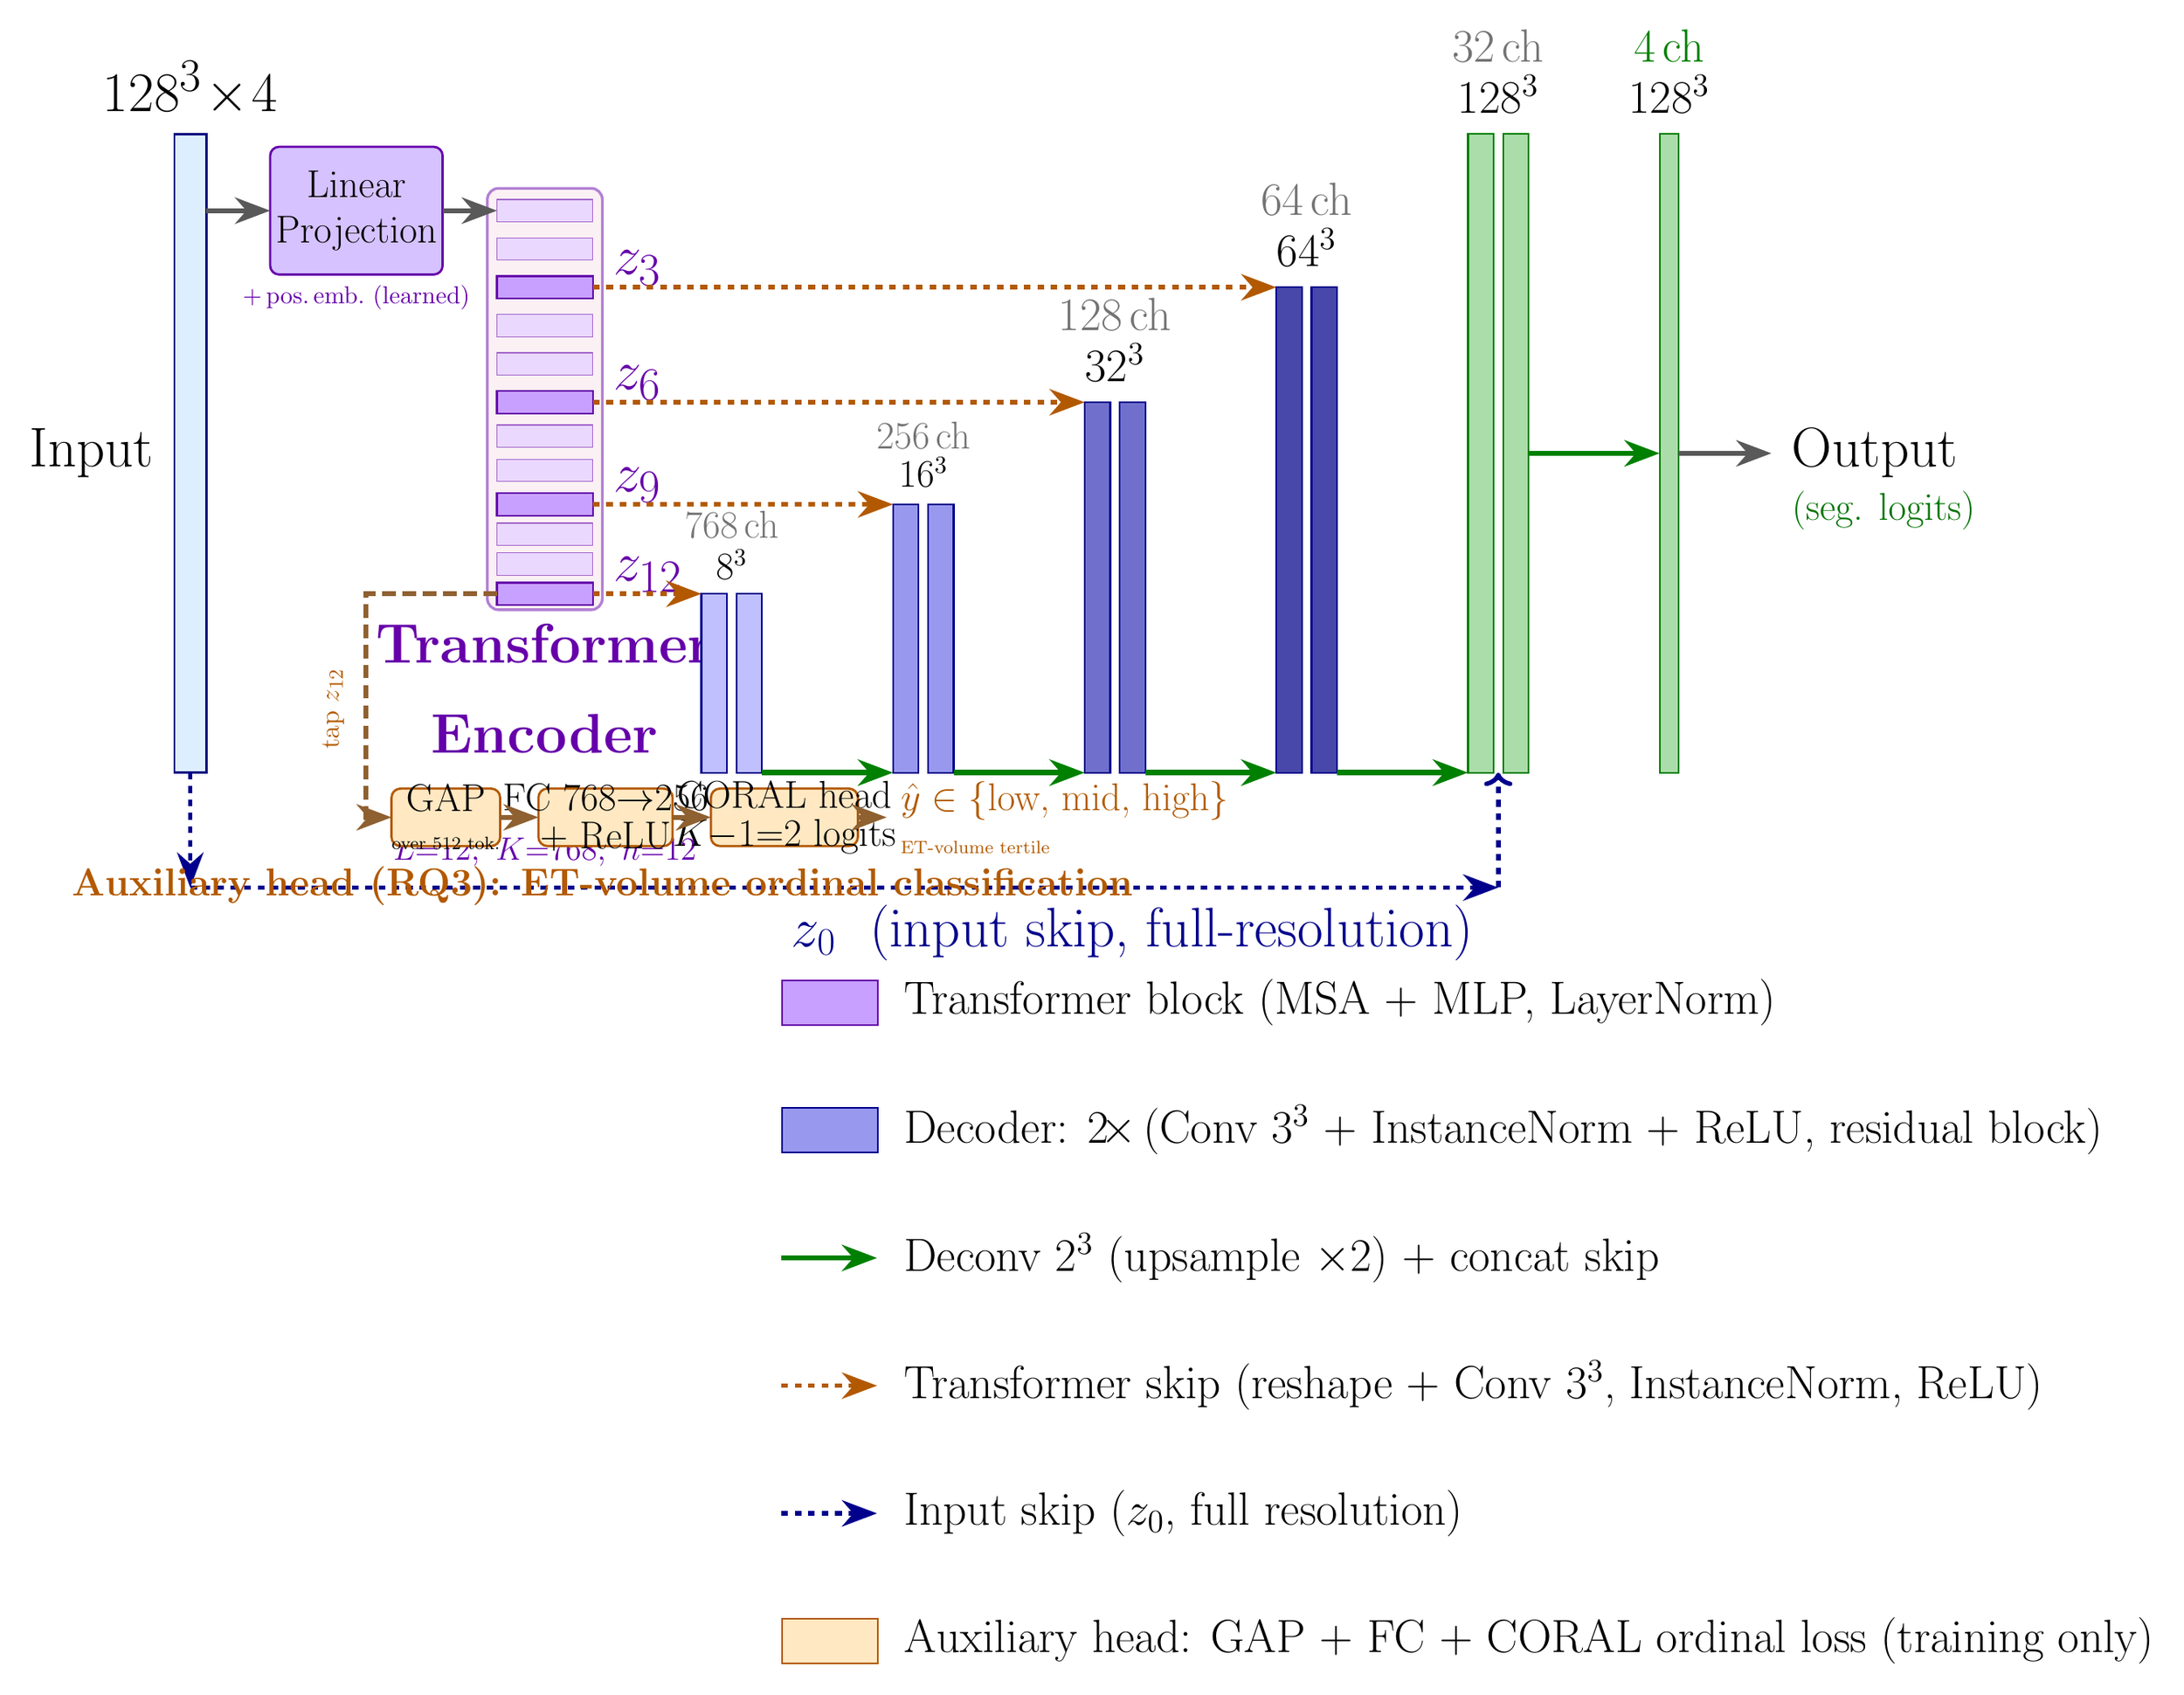
\begin{tikzpicture}[
  font=\fontsize{35}{42}\selectfont,
  arr/.style    = {-{Stealth[length=5.5mm]}, line width=2.2pt, draw=black!65},
  up/.style     = {-{Stealth[length=5.5mm]}, line width=2.4pt, draw=green!50!black},
  trskip/.style = {-{Stealth[length=5.5mm]}, line width=2.0pt, draw=orange!70!black, dashed},
  inskip/.style = {-{Stealth[length=5.5mm]}, line width=2.0pt, draw=blue!55!black,   dashed},
  auxarr/.style = {-{Stealth[length=5.5mm]}, line width=2.0pt, draw=brown!75!black},
  auxtap/.style = {-{Stealth[length=5.5mm]}, line width=2.0pt, draw=brown!75!black, dash pattern=on 6pt off 3pt},
]

% ── Color definitions ─────────────────────────────────────────────────────────
\definecolor{trfill}{HTML}{EAD8FF}
\definecolor{trhi}  {HTML}{C8A0FF}
\definecolor{tredge}{HTML}{6600AA}
\definecolor{emfill}{HTML}{D5C2FF}
\definecolor{dec1c} {HTML}{C0C0FF}
\definecolor{dec2c} {HTML}{9898EE}
\definecolor{dec3c} {HTML}{7070CC}
\definecolor{dec4c} {HTML}{4848AA}
\definecolor{dec5c} {HTML}{AADDAA}
\definecolor{infill}{HTML}{DDEEFF}
\definecolor{auxfill}{HTML}{FFE8C2}
\definecolor{auxedge}{HTML}{B25900}

% ── Decoder stage macro (bottom-aligned at YBOT = -1.6) ──────────────────────
\newcommand{\mkdec}[5]{%
  \filldraw[fill=#4, draw=#5, line width=0.8pt]
    (#2, -1.6) rectangle ++(0.40, {#3});
  \filldraw[fill=#4, draw=#5, line width=0.8pt]
    ({#2+0.55}, -1.6) rectangle ++(0.40, {#3});
  \coordinate (#1-bl)  at (#2,        -1.6);
  \coordinate (#1-br)  at ({#2+0.95}, -1.6);
  \coordinate (#1-tl)  at (#2,        {-1.6+#3});
  \coordinate (#1-tr)  at ({#2+0.95}, {-1.6+#3});
  \coordinate (#1-ml)  at (#2,        {-1.6+#3/2});
  \coordinate (#1-mr)  at ({#2+0.95}, {-1.6+#3/2});
  \coordinate (#1-tc)  at ({#2+0.475},{-1.6+#3});
  \coordinate (#1-bc)  at ({#2+0.475},-1.6);
}

% ── Auxiliary-head box macro: \mkaux{name}{x_left}{width}{line1}{line2} ───────
% Box vertically centred at y=-2.3, half-height 0.45 (so y in [-2.75,-1.85]).
\newcommand{\mkaux}[5]{%
  \filldraw[fill=auxfill, draw=auxedge, line width=1.0pt, rounded corners=4pt]
    (#2, -2.75) rectangle ++({#3}, 0.90);
  \node[align=center, font=\fontsize{16}{19}\selectfont] at ({#2+#3/2}, -2.3) {#4\\[-2pt]#5};
  \coordinate (#1-l) at (#2,        -2.3);
  \coordinate (#1-r) at ({#2+#3},   -2.3);
}

% ── Input block (x=0, w=0.50, y=-1.6 to 8.4 = height 10.0) ──────────────────
\filldraw[fill=infill, draw=blue!50!black, line width=1.0pt]
  (0.0, -1.6) rectangle ++(0.50, 10.0);
\node[anchor=east] at (-0.2, 3.4) {Input};
\node[font=\fontsize{28}{34}\selectfont, anchor=south] at (0.25, 8.55)
  {$128^3\!\times\!4$};

% ── Patch embedding box ────────────────────────────────────────────
\filldraw[fill=emfill, draw=tredge, line width=1.0pt, rounded corners=4pt]
  (1.5, 6.2) rectangle ++(2.7, 2.0);
\node[align=center, font=\fontsize{18}{22}\selectfont] at (2.85, 7.2)
  {Linear\\[-2pt]Projection};
\node[font=\fontsize{11}{13}\selectfont, color=tredge, anchor=north, align=center]
  at (2.85, 6.15) {$+$\,pos.\,emb.\ (learned)};

\draw[arr] (0.50, 7.2) -- (1.50, 7.2);
\draw[arr] (4.2, 7.2) -- (5.05, 7.2);

% ── Transformer encoder column ────────────────────────────────────────────────
\begin{pgfonlayer}{background}
  \filldraw[fill=purple!6, draw=tredge!50, line width=1.2pt, rounded corners=5pt]
    (4.9, 0.95) rectangle (6.7, 7.55);
\end{pgfonlayer}

\foreach \yc in {7.2, 6.6, 5.4, 4.8, 3.667, 3.133, 2.133, 1.667}{
  \filldraw[fill=trfill, draw=tredge!60, line width=0.5pt]
    (5.05, {\yc-0.175}) rectangle (6.55, {\yc+0.175});
}
\foreach \yc in {6.0, 4.2, 2.6, 1.2}{
  \filldraw[fill=trhi, draw=tredge, line width=0.8pt]
    (5.05, {\yc-0.175}) rectangle (6.55, {\yc+0.175});
}

\node[color=tredge, anchor=north, align=center] at (5.8, 0.85) {%
  {\fontsize{25}{30}\selectfont\bfseries Transformer}\\[-2pt]%
  {\fontsize{25}{30}\selectfont\bfseries Encoder}\\[6pt]%
  {\fontsize{14}{17}\selectfont\normalfont $L{=}12,\ K{=}768,\ h{=}12$}};

% ── Extraction labels z3, z6, z9, z12 (right of transformer) ─────────────────
\node[font=\fontsize{28}{34}\selectfont\bfseries, color=tredge, anchor=west]
  at (6.75, 6.3) {$z_3$};
\node[font=\fontsize{28}{34}\selectfont\bfseries, color=tredge, anchor=west]
  at (6.75, 4.5) {$z_6$};
\node[font=\fontsize{28}{34}\selectfont\bfseries, color=tredge, anchor=west]
  at (6.75, 2.9) {$z_9$};
\node[font=\fontsize{28}{34}\selectfont\bfseries, color=tredge, anchor=west]
  at (6.75, 1.5) {$z_{12}$};

% ── Decoder blocks ────────────────────────────────────────────────────────────
\mkdec{d1}{ 8.25}{2.80}{dec1c}{blue!55!black}
\mkdec{d2}{11.25}{4.20}{dec2c}{blue!55!black}
\mkdec{d3}{14.25}{5.80}{dec3c}{blue!55!black}
\mkdec{d4}{17.25}{7.60}{dec4c}{blue!55!black}
\mkdec{d5}{20.25}{10.0}{dec5c}{green!50!black}

\filldraw[fill=dec5c, draw=green!50!black, line width=0.8pt]
  (23.25, -1.6) rectangle ++(0.30, 10.0);
\coordinate (out-ml) at (23.25, 3.4);
\coordinate (out-mr) at (23.55, 3.4);

\node[anchor=west] at (25.2, 3.4) {Output};
\node[font=\fontsize{16}{20}\selectfont, anchor=west, color=green!45!black]
  at (25.2, 2.5) {(seg. logits)};
\draw[arr] (out-mr) -- (25.0, 3.4);

% ── Decoder block labels ──────────────────────────────────────────────────────
\node[font=\fontsize{16}{20}\selectfont, anchor=south] at ( 8.725, 1.3) {$8^3$};
\node[font=\fontsize{16}{20}\selectfont, anchor=south, color=black!55] at ( 8.725, 1.95) {768\,ch};
\node[font=\fontsize{16}{20}\selectfont, anchor=south] at (11.725, 2.75) {$16^3$};
\node[font=\fontsize{16}{20}\selectfont, anchor=south, color=black!55] at (11.725, 3.35) {256\,ch};
\node[font=\fontsize{22}{27}\selectfont, anchor=south] at (14.725, 4.4) {$32^3$};
\node[font=\fontsize{22}{27}\selectfont, anchor=south, color=black!55] at (14.725, 5.2) {128\,ch};
\node[font=\fontsize{22}{27}\selectfont, anchor=south] at (17.725, 6.2) {$64^3$};
\node[font=\fontsize{22}{27}\selectfont, anchor=south, color=black!55] at (17.725, 7.0) {64\,ch};
\node[font=\fontsize{22}{27}\selectfont, anchor=south] at (20.725, 8.6) {$128^3$};
\node[font=\fontsize{22}{27}\selectfont, anchor=south, color=black!55] at (20.725, 9.4) {32\,ch};
\node[font=\fontsize{22}{27}\selectfont, anchor=south] at (23.40,  8.6) {$128^3$};
\node[font=\fontsize{22}{27}\selectfont, anchor=south, color=green!50!black] at (23.40, 9.4) {4\,ch};

% ── Transformer skip connections ──────────────────────────────────────────────
\draw[trskip] (6.55, 6.0) -- (d4-tl);
\draw[trskip] (6.55, 4.2) -- (d3-tl);
\draw[trskip] (6.55, 2.6) -- (d2-tl);
\draw[trskip] (6.55, 1.2) -- (d1-tl);

% ── Upsample arrows ───────────────────────────────────────────────────────────
\draw[up] (d1-br) -- (d2-bl);
\draw[up] (d2-br) -- (d3-bl);
\draw[up] (d3-br) -- (d4-bl);
\draw[up] (d4-br) -- (d5-bl);
\draw[up] (d5-mr) -- (out-ml);

% ── Input skip z0 (route below figure) ───────────────────────────────────────
\draw[inskip] (0.25, -1.6) -- (0.25, -3.4);
\draw[inskip] (0.25, -3.4) -- (20.725, -3.4);
\draw[inskip, ->] (20.725, -3.4) -- (20.725, -1.6);
\node[font=\fontsize{25}{30}\selectfont, color=blue!55!black, anchor=north]
  at (15.0, -3.55) {$z_0$\ \ (input skip, full-resolution)};

% ═══════════════════════════════════════════════════════════════════════════
% ── AUXILIARY HEAD (RQ3): ET-volume ordinal classification ──────────────────
% Tap z12 (bottleneck), GAP over the 512 tokens, then FC + CORAL ordinal head.
% Placed in the free band below the encoder, left of the decoder.
% ═══════════════════════════════════════════════════════════════════════════
\mkaux{gap}  {3.40}{1.70}{GAP}{\footnotesize over 512 tok.}
\mkaux{fc}   {5.70}{2.10}{FC $768{\to}256$}{$+$ ReLU}
\mkaux{coral}{8.40}{2.30}{CORAL head}{$K{-}1{=}2$ logits}

% Tap from z12: left out of the encoder (y=1.2, above the label), then down.
\draw[auxtap] (5.05, 1.2) -- (3.0, 1.2) -- (3.0, -2.3) -- (gap-l);
\node[font=\fontsize{13}{16}\selectfont, color=auxedge, anchor=south, rotate=90]
  at (2.78, -0.6) {tap $z_{12}$};

% Inter-stage arrows
\draw[auxarr] (gap-r)   -- (fc-l);
\draw[auxarr] (fc-r)    -- (coral-l);
\draw[auxarr] (coral-r) -- ++(0.45, 0);

% Ordinal output
\node[font=\fontsize{16}{20}\selectfont, color=auxedge, anchor=west, align=left]
  at (11.25, -2.3) {$\hat{y}\in\{$low, mid, high$\}$\\[-1pt]{\footnotesize ET-volume tertile}};

% Auxiliary-head group label
\node[font=\fontsize{17}{21}\selectfont\bfseries, color=auxedge, anchor=north]
  at (6.7, -2.95) {Auxiliary head (RQ3): ET-volume ordinal classification};

% ── Legend ────────────────────────────────────────────────────────────────────
\def\LY{-5.2}
\def\LS{2.0}
\def\LXLEG{9.5}

\node[draw=tredge, fill=trhi, line width=0.7pt,
      minimum width=1.5cm, minimum height=0.7cm, anchor=west] at (\LXLEG, \LY) {};
\node[font=\fontsize{20}{24}\selectfont, anchor=west] at ({\LXLEG+1.8}, \LY)
  {Transformer block (MSA $+$ MLP, LayerNorm)};

\node[draw=blue!55!black, fill=dec2c, line width=0.7pt,
      minimum width=1.5cm, minimum height=0.7cm, anchor=west] at (\LXLEG, {\LY-\LS}) {};
\node[font=\fontsize{20}{24}\selectfont, anchor=west] at ({\LXLEG+1.8}, {\LY-\LS})
  {Decoder: $2\!\times\!$ (Conv $3^3$ $+$ InstanceNorm $+$ ReLU, residual block)};

\draw[up] (\LXLEG, {\LY-2*\LS}) -- ++(1.5, 0);
\node[font=\fontsize{20}{24}\selectfont, anchor=west] at ({\LXLEG+1.8}, {\LY-2*\LS})
  {Deconv $2^3$ (upsample $\times 2$) $+$ concat skip};

\draw[trskip] (\LXLEG, {\LY-3*\LS}) -- ++(1.5, 0);
\node[font=\fontsize{20}{24}\selectfont, anchor=west] at ({\LXLEG+1.8}, {\LY-3*\LS})
  {Transformer skip (reshape $+$ Conv $3^3$, InstanceNorm, ReLU)};

\draw[inskip] (\LXLEG, {\LY-4*\LS}) -- ++(1.5, 0);
\node[font=\fontsize{20}{24}\selectfont, anchor=west] at ({\LXLEG+1.8}, {\LY-4*\LS})
  {Input skip ($z_0$, full resolution)};

\node[draw=auxedge, fill=auxfill, line width=0.7pt,
      minimum width=1.5cm, minimum height=0.7cm, anchor=west] at (\LXLEG, {\LY-5*\LS}) {};
\node[font=\fontsize{20}{24}\selectfont, anchor=west] at ({\LXLEG+1.8}, {\LY-5*\LS})
  {Auxiliary head: GAP $+$ FC $+$ CORAL ordinal loss (training only)};

\end{tikzpicture}
\end{document}
